\subsubsection*{Estructuras del Scheduler}
\par Las variables de nuestro scheduler son las siguientes:

\begin{lstlisting} [caption={Variables del Scheduler},label=SchedulerVars]
info_player playerA;
info_player playerB;
int playerActual;
int isIdle;
\end{lstlisting}

\par $playerActual$ indica cu\'al es el jugador que tiene el turno actualmente; $info\_playerA$ e $info\_playerB$ guardan la informaci\'on relevante al jugador. Finalmente, nos pareci\'o relevante agregar la variable $isIdle$, que indica si la tarea actual es la Idle.

\begin{lstlisting} [caption={Informaci\'on del zombi},label=infoZombi]
typedef struct str_info_zombie {
    zombie  type;
    unsigned short  x;
    unsigned short  y;
    unsigned short reloj_actual;
} __attribute__((__packed__, aligned (16))) info_zombie;
\end{lstlisting}

\par \texttt{info_zombie} guarda su posici\'on actual la pantalla, su tipo (que es un enum), y su reloj actual (que es un n\'umero entre 0 y 3 que indica qu\'e caracter del reloj tiene dibujado el zombi en este momento). 

\begin{lstlisting} [caption={Informaci\'on del jugador},label=infoPlayer]
typedef struct str_info_player {
    zombie  selected_type;
    unsigned short  y;
    unsigned short cant_lanzados;
    unsigned short gdt_indexes_tasks[CANT_ZOMBIS];
    info_zombie info_zombies[CANT_ZOMBIS];
    unsigned short curr_zombie;
    unsigned short puntos;
} __attribute__((__packed__, aligned (16))) info_player;
\end{lstlisting}

\par Por otro lado, \texttt{info_player} guarda el tipo de zombie seleccionado actualmente, la posici\'on del jugador en el eje vertical, la cantidad de zombies lanzados, y sus puntos. Lo m\'as interesante es \texttt{gdt_indexes_tasks} que es un arreglo de selectores de la gdt, donde el i-\'esimo selector se corresponde con el i-\'esimo zombie de info\_zombies. Por \'ultimo, curr\_zombie indica el \'indice del zombie actual del jugador.

\newpage

\subsubsection*{Task switch}

\par{Como vemos en la figura 3, las tareas de los zombies deben ir alternandose entre el jugador A y el B. Adem\'as los zombies de cada jugador deben correr uno tras otro y de manera c\'iclica.}

\begin{figure}[ht!]
\centering
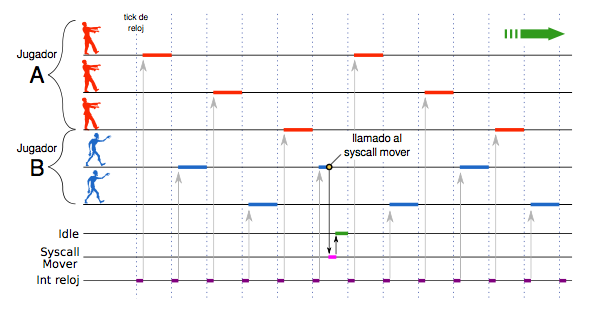
\includegraphics[width=100mm]{imagenes/scheduler.png}
\caption{Ejemplo de funcionamiento del Scheduler}
\end{figure}

\par{Lo que hacemos entonces es preguntar en cada interrupci\'on de reloj qui\'en es el pr\'oximo \'indice de tarea a ejecutar y hacemos el jump a ella. En caso que el scheduler nos devuelva el \'indice 0 no haremos nada, nos quedamos en la tarea actual. A continuaci\'on el c\'odigo de la interrupci\'on de clock.}

\begin{lstlisting} [caption={Interrupci\'on de clock},label=infoPlayer]
_isr32:
    pushad

    call proximo_reloj
    mov eax, [inDebugMode] 
    mov esi, [debugScreenOpen]
    and eax, esi
    cmp eax, 1
    je .nojump  ;si esta en modo debug con la pantalla de debug abierta no hago nada


    call sched_proximo_indice

    cmp ax, 0
    je .nojump
        push eax
        call girar_reloj_actual
        pop eax
        mov [selector], ax
        call fin_intr_pic1
        jmp far [offset]
        jmp .end

    .nojump:
    call fin_intr_pic1

    .end:
    popad
    iret
\end{lstlisting}

\\
\par{Nos salteamos las lineas que hablan del debugger ya que este ser\'a explicado m\'as adelante. Como vemos hacemos un $call$ a $sched\_proximo\_indice$ como habiamos dicho y a continuaci\'on saltamos a esa tarea. En caso de ser 0 no hacemos ning\'un $jmp$.}
\par{Lo que hace $sched\_proximo\_indice$ es tomar la informaci\'on de playerActual para saber quien es el siguiente jugador. Si el jugador opuesto al actual no tiene tareas en su lista de $gdt\_index\_tasks$ (osea tiene todos 0), entonces no se cambiar\'a el $playerActual$. En caso contrario, el player actual pasar\'a a el otro jugador.}
\par{Si este es el primer zombie que se lanza (caso en que zombie inicial del player ser\'a 32) entonces verifico que haya zombies en la lista de indices, puesto que si no los hay es por que a\'un no se han lanzado zombies y por ende no hay que saltar a ninguna tarea de este jugador. Si hay zombies en la lista entonces el primer zombie ser\'a el proximo a saltar.}
\par{Si no estamos en el caso anterior entonces lo que hay que hacer es recorrer la lista de \'indices busucando el primero que sea distinto de 0. Si se llega al final del arreglo se empieza desde el inicio. Si se encuentra de esta manera una tarea distinta a la actual para este jugador entonces ser\'a ese \'indice el que se devuelva y esa tarea a la que se salte.}
\par{Si se dio toda la vuelta y se lleg\'o al mismo zombie que el actual entonces tenemos que preguntarnos si estamos en la tarea Idle ya que si estamos en la tarea idle entonces vuelve a ser el turno de este zombie, pero si no estamos en la tarea idle entonces no debemos hacer nada y devolver 0 ya que actualmente estamos en el turno de ese zombie.}



\newpage
\subsubsection*{Syscall mover}

\par La syscall mover es la \'unica prove\'ida por el sistema, y est\'a mapeada a la interrupci\'on 0x66.
\par La codificaci\'on de desplazamientos es la siguiente:

\begin{figure}[ht!]
\centering
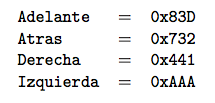
\includegraphics[width=40mm]{imagenes/movercodes.png}
\caption{C\'odigos de mover}
\end{figure}

\par Atendemos la interrupci\'on en assembler y llamamos a \texttt{game_move_current_zombi} en C, cuyo \'unico par\'ametro es la direcci\'on en la que quiere moverse el zombie, y su funcionamiento es:

\begin{itemize}
\item 1. Dada la direcci\'on pasada por par\'ametro, obtenemos la p\'agina virtual a donde se va a mover.
\end{itemize}

\begin{lstlisting} [caption={Syscall mover - obtener origen y destino},label=moverOrigen]
    unsigned int* orig = (unsigned int*) VIRTUAL_COD_ZOMBIE_1;
    unsigned int* dest;
	switch (dir) {
	case IZQ:
    	dest = (unsigned int*)VIRTUAL_COD_ZOMBIE_6;
		break;
    case DER:
    	dest = (unsigned int*)VIRTUAL_COD_ZOMBIE_5; 
    	break;
    case ADE:
    	dest = (unsigned int*)VIRTUAL_COD_ZOMBIE_2;
    	break;
    case ATR:
    	dest = (unsigned int*)VIRTUAL_COD_ZOMBIE_7;    
    	break;
    }
\end{lstlisting}

\begin{itemize}
\item 2. Copiamos la p\'agina entera del c\'odigo del zombie, a su p\'agina f\'isica de destino. Esto es copiando su p\'agina virtual actual a su p\'agina virtual destino, porque ambas est\'an mapeadas sus correspondientes f\'isicas.
\end{itemize}

\begin{lstlisting} [caption={Syscall mover - copiar c\'odigo del zombie},label=moverCopiar]
    int i;
    for(i=0; i<1024; i++){
    	dest[i] = orig[i];
    }
\end{lstlisting}

\begin{itemize}
\item 3. Calculamos la nueva posici\'on (x, y) (tomando en cuenta qu\'e jugador es el actual, y la circularidad del mapa).
\end{itemize}

\begin{lstlisting} [caption={Syscall mover - calcular nueva (x, y)},label=moverNuevaXY]
info_player* current_player = get_current_player();
    unsigned short current_zombie = current_player->curr_zombie;
    unsigned short x_orig = (current_player->info_zombies[current_zombie]).x;
    unsigned short y_orig = (current_player->info_zombies[current_zombie]).y;
    unsigned short x_dst = x_orig;
    unsigned short y_dst = y_orig;

    if(y_dst==0 || y_dst==43){
        if ((dir == IZQ && playerActual == 0) || (dir == DER && playerActual == 1)) {
            y_dst=43;
        } else if ((dir == DER && playerActual == 0) || (dir == IZQ && playerActual == 1)) {
            y_dst=0;
        } else if ((dir == ADE && playerActual == 0) || (dir == ATR && playerActual == 1)) {
            x_dst++;

        } else if ((dir == ATR && playerActual == 0) || (dir == ADE && playerActual == 1)) {
            x_dst--;
        }
    }else{
        if ((dir == IZQ && playerActual == 0) || (dir == DER && playerActual == 1)) {
            y_dst--;
        } else if ((dir == DER && playerActual == 0) || (dir == IZQ && playerActual == 1)) {
            y_dst++;
        } else if ((dir == ADE && playerActual == 0) || (dir == ATR && playerActual == 1)) {
            x_dst++;

        } else if ((dir == ATR && playerActual == 0) || (dir == ADE && playerActual == 1)) {
            x_dst--;
        }
    }   

\end{lstlisting}

\begin{itemize}
\item 4. Asignamos al zombie a su nueva posici\'on.
\end{itemize}

\begin{lstlisting} [caption={Syscall mover - asignar nuevas coordenadas al zombie},label=moverAsignarCoordenadas]
    (current_player->info_zombies[current_zombie]).x = x_dst;
    (current_player->info_zombies[current_zombie]).y = y_dst;
\end{lstlisting}

\begin{itemize}
\item 5. De llegar a un borde, sumamos punto, matamos al zombie, y terminamos la ejecuci\'on del algoritmo.
\end{itemize}

\begin{lstlisting} [caption={Syscall mover - sumar punto y matar zombie},label=moverSumarYMatar]
    if(x_dst==1){
        game_sumar_punto(1/*jugador azul*/);
        game_matar_zombie_actual();
        return;
    }
    if(x_dst==78){
        game_sumar_punto(0/*jugador rojo*/);
        game_matar_zombie_actual();
        return;
    }
\end{lstlisting}

\begin{itemize}
\item 6. Remapeamos todas las p\'aginas virtuales del zombie teniendo en cuenta su nueva posici\'on (x, y).
\end{itemize}

\begin{lstlisting} [caption={Syscall mover - remapear las p\'aginas del zombie (vease Ej. 4)},label=moverRemapear]
    /* remapear sus direcciones */
    mmu_map_adjacent_to_zombi(playerActual, rcr3(), x_dst, y_dst);
\end{lstlisting}

\begin{itemize}
\item 7. Por \'ultimo imprimimos el cambio en pantalla y seteamos la tarea idle en el scheduler.
\end{itemize}

\begin{lstlisting} [caption={Syscall mover - Imprimir en pantalla y setear Idle},label=moverImprimir]
    print_move_zombie(playerActual, x_orig, y_orig, x_dst, y_dst, (current_player->info_zombies[current_zombie]).type);
    isIdle=1;
\end{lstlisting}

\subsubsection*{Modo debug}
\par{Para implementar el modo debug en nuestro juego nos encontramos con tres problem\'aticas:}
\begin{enumerate}
\item C\'omo recuperar los valores de algunos registros que son modificados cuando se produce la interrupci\'on
\item Guardar el estado de la pantalla del juego antes de que aparezca el cartel, para luego poder restaurarla
\item Que otras tareas no se sigan ejecutando y que los jugadores no puedan realizar acciones cuando esta la pantalla de debug abierta
\end{enumerate}

\par{Para guardar el estado de los registros al momento de producirse una interrupci\'on contamos con el struct debug_info. La mayor\'ia de los registros siguen iguales despu\'es de producida la interrupci\'on. Algunos son modificados, pero antes son apilados en el stack. El estado del stack despues de transferir el control al handler de interrupciones es el siguiente:}

\begin{figure}[ht!]
\centering
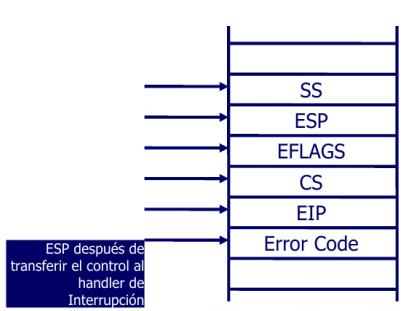
\includegraphics[width=70mm]{imagenes/stack.png}
\caption{Stack al momento de entrar al handler de interrupciones}
\end{figure}

\par{Por otro lado, para poder guardar el estado de la pantalla antes de que aparezca el cartel del debugger contamos con la variable $backup$ (matriz de $ca$ que se corresponde con la pantalla), la funci\'on $backup\_screen$ (que guarda la pantalla en la variable) y la funci\'on $backup\_restore\_screen$ (que escribe en la pantalla lo que hay guardado en la variable).}

\par{Por \'ultimo, para poder manejar las tareas en modo debug contamos con dos variables globales: inDebugMode, que indican si se est\'a en modo debug, y $debugScreenOpen$, que indica si la ventana de debug est\'a abierta. Al producirse la excepci\'on se setea $debugSreenOpen$ en 1, se muestra la pantalla de debug y se salta a la tarea Idle. Dentro de la interrupci\'on de clock, si $inDebugMode$ y $debugScreenOpen$ est\'an seteados, no se salta a la pr\'oxima tarea. Dentro de la interrupci\'on de teclado, si $inDebugMode$ y $debugScreenOpen$ est\'an seteados, solamente la tecla 'y' produce un cambio en el juego (cerrar la pantalla de debug).}